\chapter{実装}
\label{chap:implementation}

\section{実装概要}

第\ref{chap:design}章でも述べた通り、本研究では「インスリンペンを使用してインスリンが摂取された時間」と「患者本人が食事を開始した時間」を取得するため、それぞれのデバイスが必要である。
本章では、それぞれの実装内容について触れる。

\section{インスリンペンデバイス}
\label{section:insulin_pen_device}

\subsection{環境}

インスリン摂取を検知するためのインスリンペンデバイスは以下の機器で構成される。

\begin{table}[htbp]
  \caption{インスリンデバイスの実装環境}
  \label{tb:insulin-device}
  \begin{center}
    \begin{tabular}{|c||c|}
      \hline
      開発言語  & C++ \\\hline
      通信機器  & ESP32 devkit v1(図\ref{fig:esp32}) \\\hline
      注射器を模したもの & マッキーペン (図\ref{fig:insulin_pen})\\\hline
    \end{tabular}
  \end{center}
\end{table}

\begin{figure}[htbp]
  \caption{今回使用したESP32 devkit v1}
  \label{fig:esp32}
  \begin{center}
    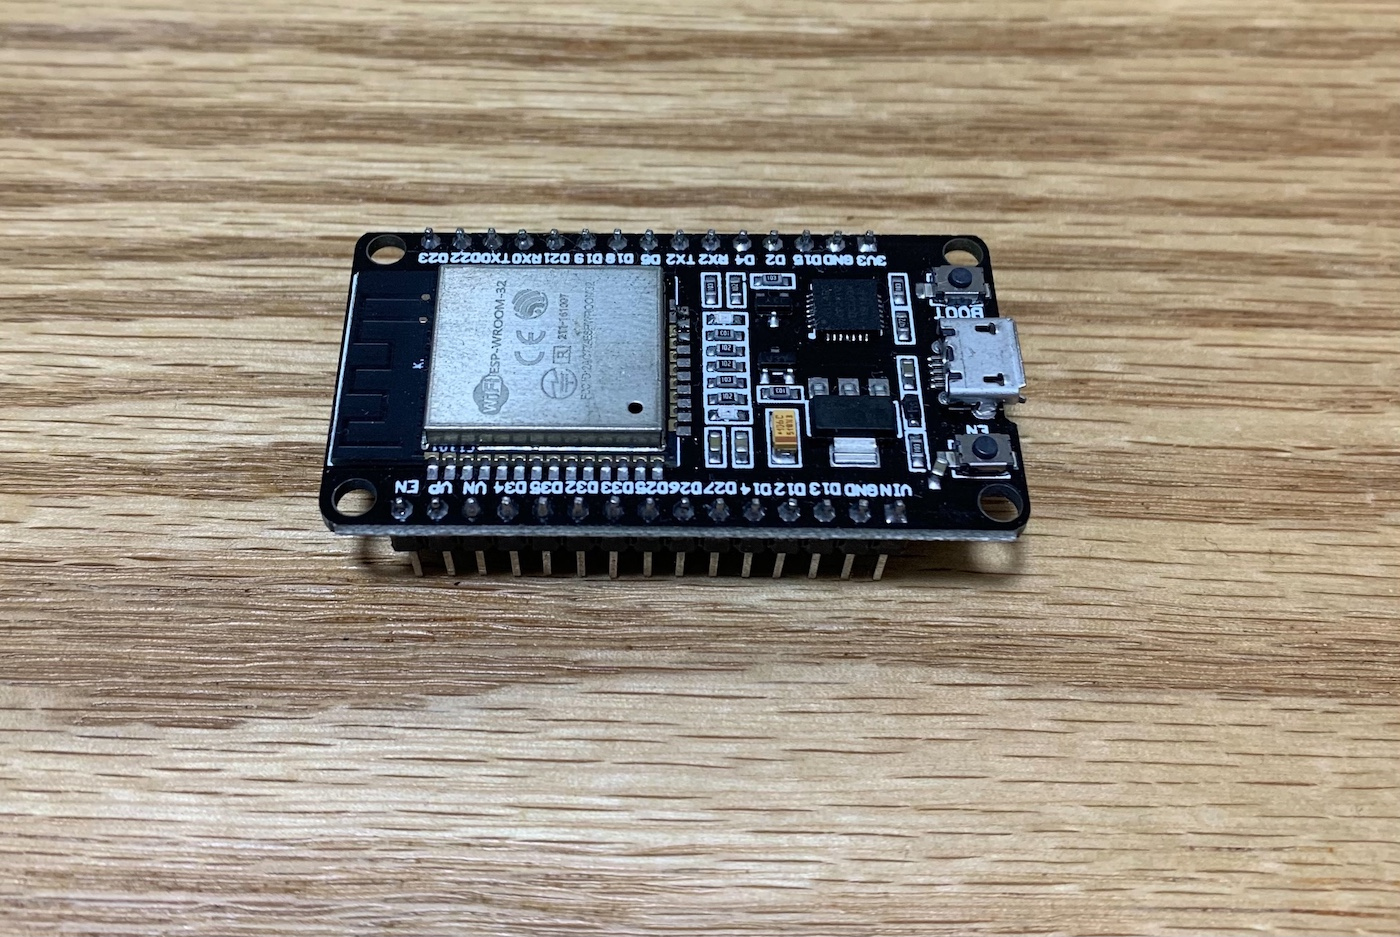
\includegraphics[bb=0 0 1300 1100,width=10cm]{assets/esp32.jpg}
  \end{center}
\end{figure}

\begin{figure}[htbp]
  \caption{今回使用したインスリン注射器}
  \label{fig:insulin_pen}
  \begin{center}
    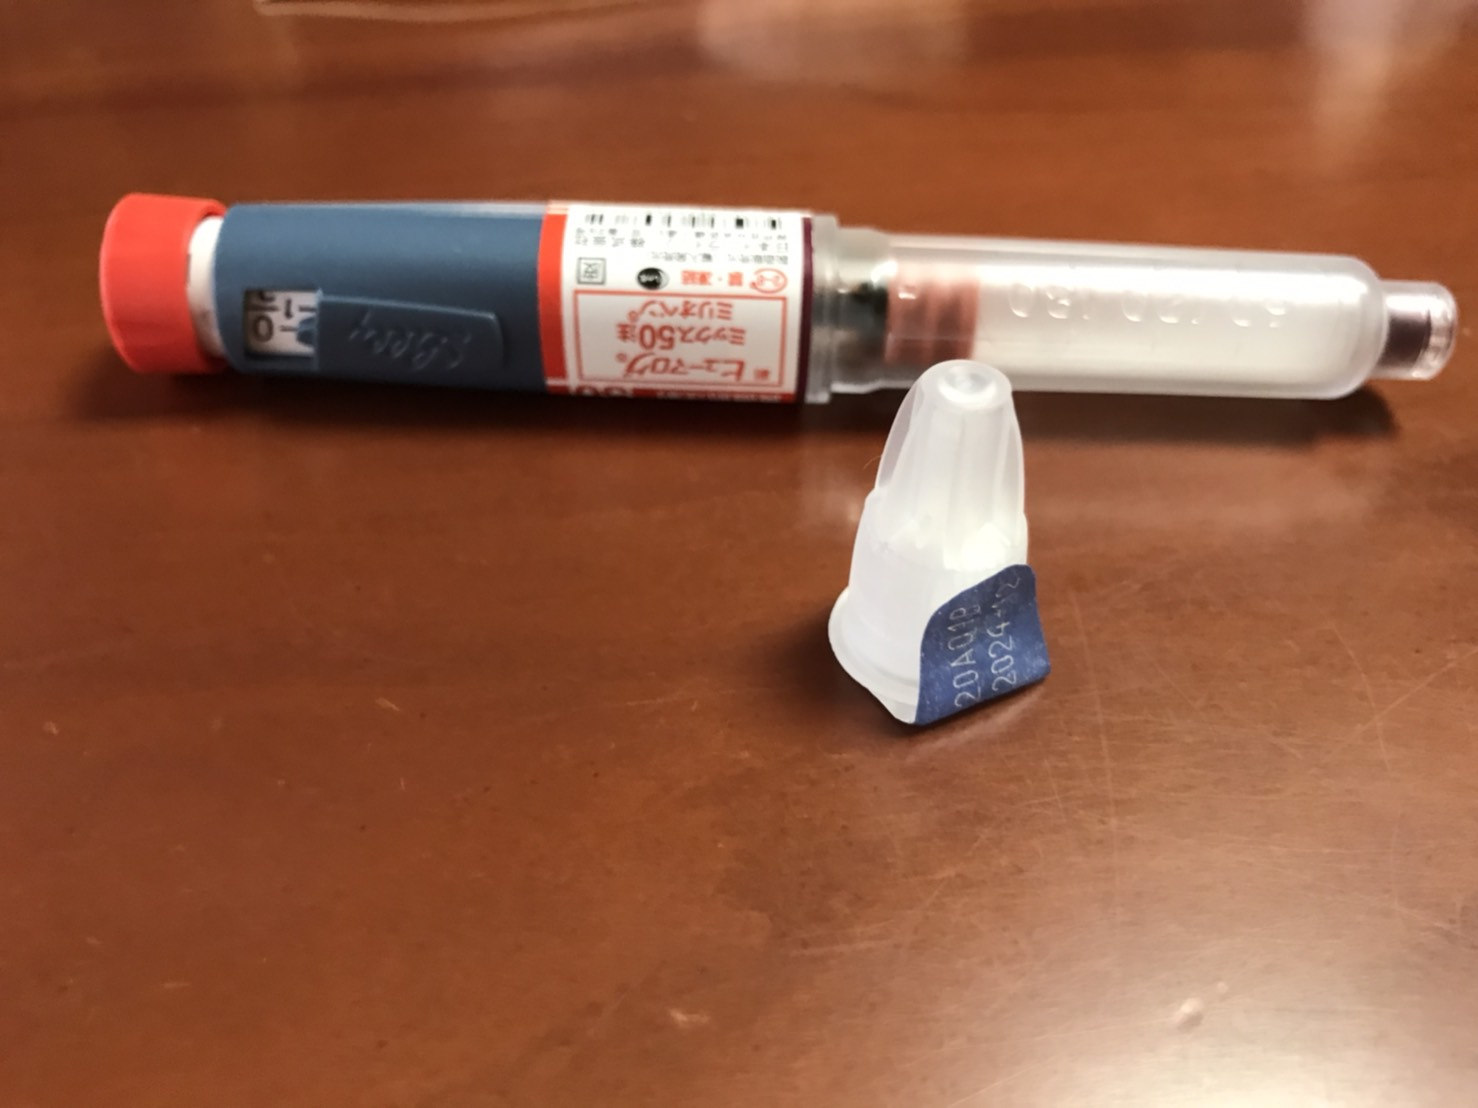
\includegraphics[bb=0 0 1300 1200,width=10cm]{assets/insulin_pen_needle.jpg}
  \end{center}
\end{figure}

インスリン注射器の端のボタンが一定時間以上押された場合に摂取と判定する構造を作るため、今回は物理的なタクタイルスイッチを接着し、このボタンが押された場合にのみ、
インスリンが摂取されたとして判定するよう実装した。

図\ref{fig:insulin_pen_device_circuit}に、ESP32とそのスイッチ回路を示す。

\begin{figure}[htbp]
  \caption{インスリン注射器に装着するデバイスの電子回路}
  \label{fig:insulin_pen_device_circuit}
  \begin{center}
    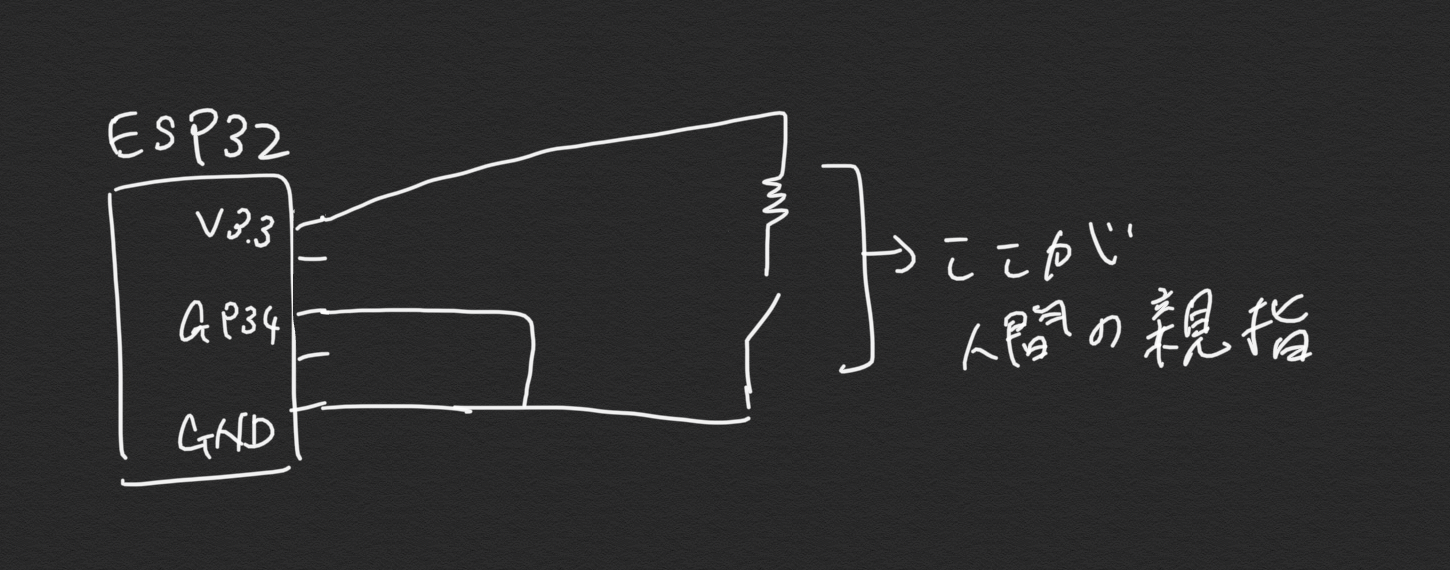
\includegraphics[bb=0 0 1000 300,width=20cm]{assets/insulin_pen_device_circuit.png}
  \end{center}
\end{figure}

配線は図\ref{}に示した。

図\ref{}が実際の実装物である。小型化し、電池により携帯可能にする段階は本研究の本質ではないため、今回の実装内容としては省いた。

図\ref{fig:insulin_injection_test}が実装したインスリンデバイスを使った時の電流の変化である。
横軸を時刻、縦軸をデジタル読み取りの0,1で取った。

\begin{figure}[htbp]
  \caption{インスリン検知デバイスを使った時のデジタル読み取りのデータ}
  \label{fig:insulin_injection_test}
  \begin{center}
    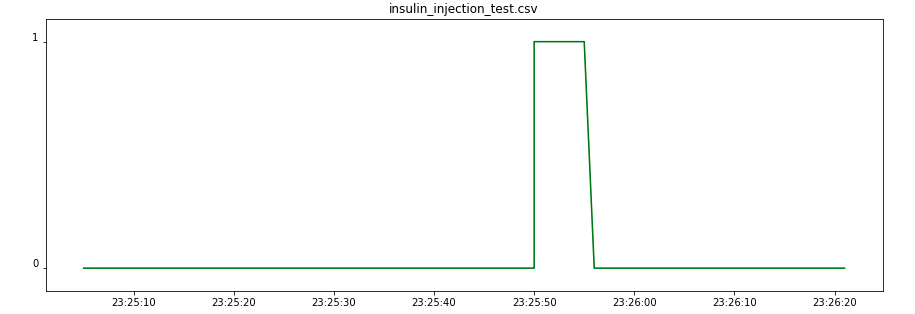
\includegraphics[bb=0 0 1000 350,width=17cm]{assets/insulin_injection_test.png}
  \end{center}
\end{figure}

ここにある通り、指によってインスリンペンの端が押下されると、一時的に電流が流れ、ESP32のpin34で電流が読み取れていることがわかる。
本研究では、この電流が一定時間以上流れた場合に、そのイベントをインスリン摂取として検知した。
今回は、検知と判定するための押下時間の閾値は5秒以上とした。\cite{how_to_inject_insulin_1} \cite{how_to_inject_insulin_2}

本インスリンデバイスは、インスリン摂取を検知すると、HTTPプロトコルのPOSTメソッドを使用して、検知時間をJSONデータとしてWebサーバーにリクエストを行う。
POSTリクエストを受け取ったサーバーは、受け取ったデータをデコードし、摂取時間のタイムスタンプを取得、MySQLに保存する。
今回使用したPOSTリクエストのBodyのデータフォーマットは以下である。
タイムスタンプにはUnix Timestampを採用した。

\begin{verbatim}
  {
    "injected_time": "1610081373"
  }
\end{verbatim}

アップロード先のWebサーバーは、食事検知に使用するRaspberry Pi上にホストした。
使用した言語、フレームワークは以下の通りである。

\begin{table}[htbp]
  \caption{Webサーバーのスペック}
  \label{tb:web_server}
  \begin{center}
    \begin{tabular}{|c||c|}
      \hline
      開発言語  & python 3.7.3 \\\hline
      フレームワーク  & Flask 1.0.2 \\\hline
      DB & MySQL ver 15.1 Distrib 10.3.25-MariaDB \\\hline
    \end{tabular}
  \end{center}
\end{table}

\ref{}にこの実装部分の概略と、フローを示す。

\section{食事検知加速度センサ}

今回、食事の検知は食卓上に鎮座させる加速度センサによる手法を採用した。検知デバイスは以下の機器で構成されている。

\subsection{環境}

\begin{table}[htbp]
  \caption{食事検知に使用したセンサー及びPC}
  \label{tb:meal_detection_spec}
  \begin{center}
    \begin{tabular}{|c||c|}
      \hline
      加速度センサー & ADXL345 \\\hline
      PC & Raspberry Pi 4 Model B (SD: 32GB) \\\hline
    \end{tabular}
  \end{center}
\end{table}

\begin{table}[htbp]
  \caption{ソフトウェア関連環境}
  \label{tb:meal_detection_spec_sw}
  \begin{center}
    \begin{tabular}{|c||c|}
      \hline
      開発言語 & Python 3.7.3 \\\hline
      使用ライブラリ &  $ time, datetime, busio, board, adafruit_adxl34x $ \\\hline
    \end{tabular}
  \end{center}
\end{table}

\begin{figure}[htbp]
  \caption{加速度センサーADXL345}
  \label{fig:adxl345}
  \begin{center}
    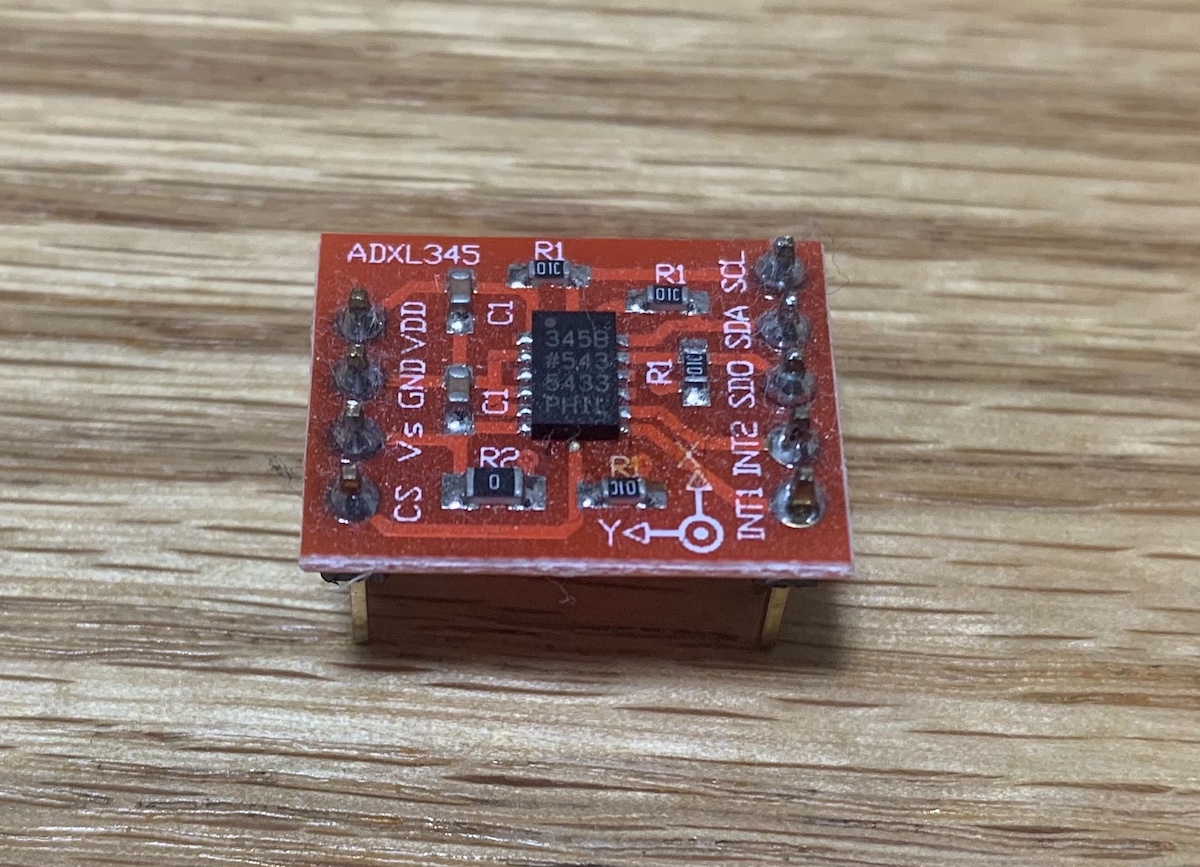
\includegraphics[bb=0 0 1300 1000,width=10cm]{assets/adxl345.jpg}
  \end{center}
\end{figure}

ADXL345は3軸加速度センサであり、縦、横、高さの3つの値を取得することができる。

\begin{figure}[htbp]
  \caption{Raspberry Pi 4 model b}
  \label{fig:raspi4_model_b}
  \begin{center}
    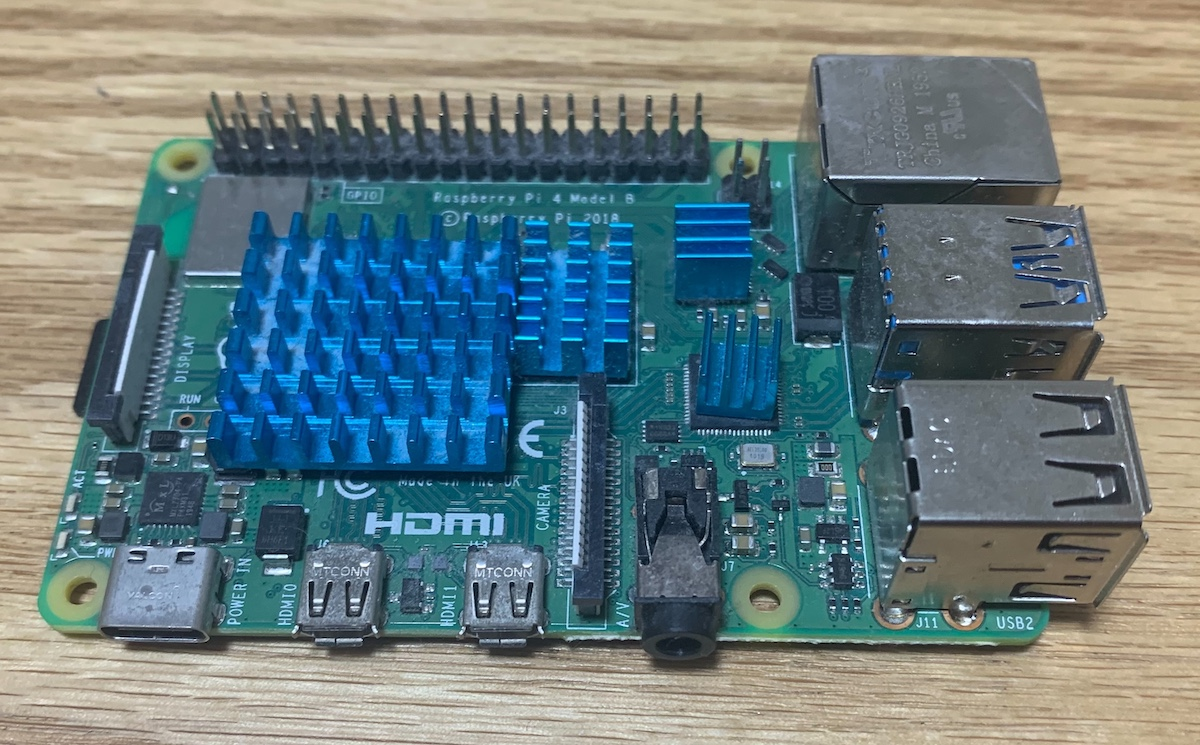
\includegraphics[bb=0 0 1300 1100,width=10cm]{assets/raspi4_model_b.jpg}
  \end{center}
\end{figure}

テーブル\ref{tb:raspberry_pi_spec}に、本研究で使用したRaspberry Piのスペックを示す。

\begin{table}[htbp]
  \caption{Raspberry Piのスペック}
  \label{tb:raspberry_pi_spec}
  \begin{center}
    \begin{tabular}{|c||c|}
      \hline
      OS  & Raspbian GNU/Linux 10 (buster) \\\hline
      CPU & Broadcom BCM2711, quad-core Cortex-A72 (ARM v8) 64-bit SoC @ 1.5GHz \\\hline
      RAM & 4GB LPDDR4-3200 SDRAM \\\hline
      Storage & Micro-SD (32GB) \\\hline
      GPIO & 40-pin GIPO header \\\hline
    \end{tabular}
  \end{center}
\end{table}

raspberry piで加速度センサの値を読めるようになるための実装説明

図\ref{fig:meal_detector_wire_illustration}に配線図を示す。

\begin{figure}[htbp]
  \caption{Raspberry Pi 4とADXL345の配線図}
  \label{fig:meal_detector_wire_illustration}
  \begin{center}
    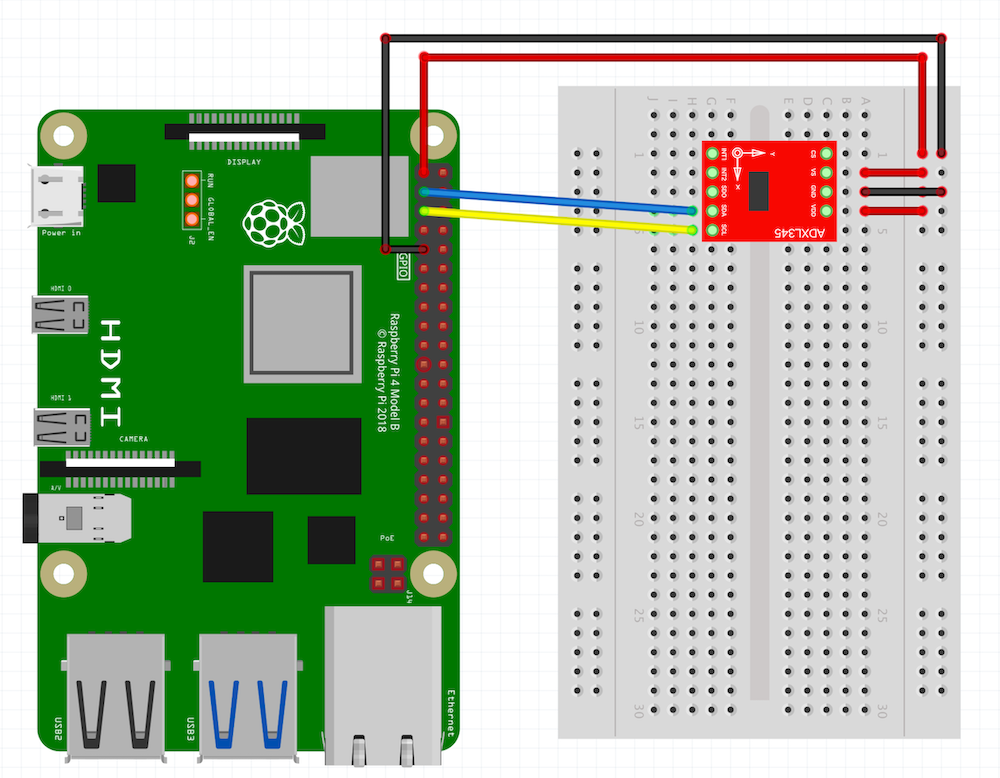
\includegraphics[bb=0 0 1000 800,width=15cm]{assets/raspi_adxl345.png}
  \end{center}
\end{figure}

そして、図\ref{fig:meal_detector}が、図\ref{fig:meeal_detector_wire_illustration}に従って配線した実物である。

\begin{figure}[htbp]
  \caption{配線したRaspberry Pi 4とADXL345}
  \label{fig:meal_detector}
  \begin{center}
    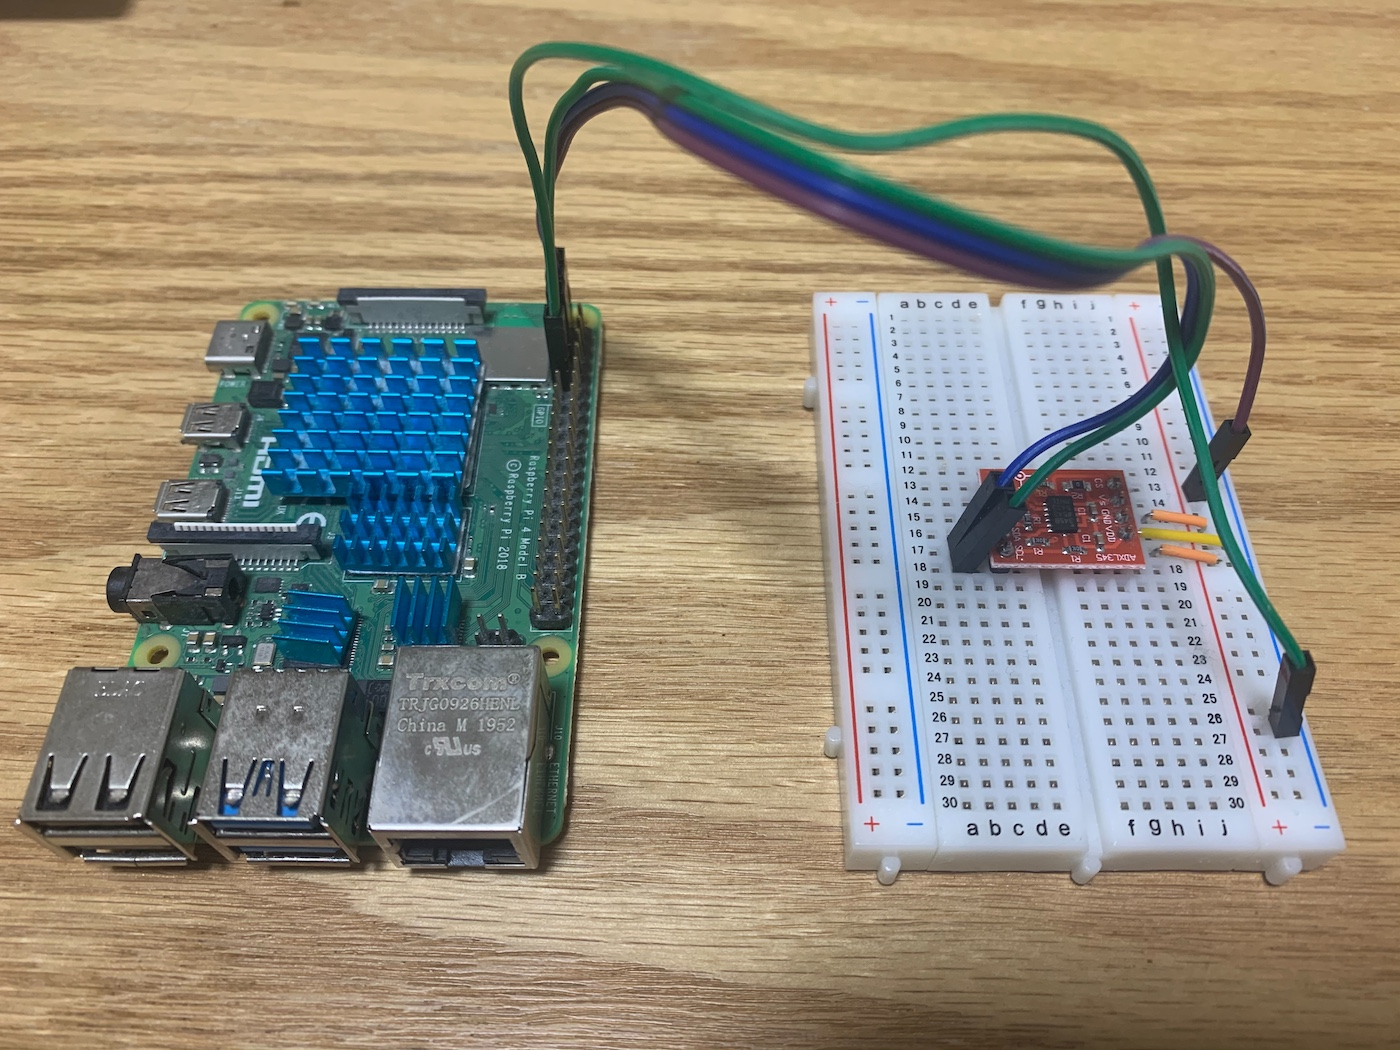
\includegraphics[bb=0 0 1300 1100,width=10cm]{assets/meal_detector.jpg}
  \end{center}
\end{figure}

加速度センサでどういう値が取れるのかをmatplotlibで可視化したやつそのまま貼って説明。

どんな条件で食事検知とするのかを書く。

\section{インスリン打ち忘れ通知}

上記で実装した、二つのデバイスから取得できたデータをもとにインスリンの打ち忘れ検知を行い、打ち忘れが起こった場合には、患者に対して通知を行う。
今回は、食事検知、Webサーバーのホストに使用したRaspberry Piにスピーカーを取り付け、そこから「You forgot your insulin injection」というセリフを流すことで、
患者に知らせる。図\ref{fig:system_flow}が、全体のフローであり、図\ref{fig:raspi_with_speaker}がスピーカーが取り付けられたRaspberry Piである。
スピーカーは〇〇を使用した。

\begin{figure}[htbp]
  \caption{インスリン摂取忘れ通知フロー}
  \label{fig:system_flow}
  \begin{center}
    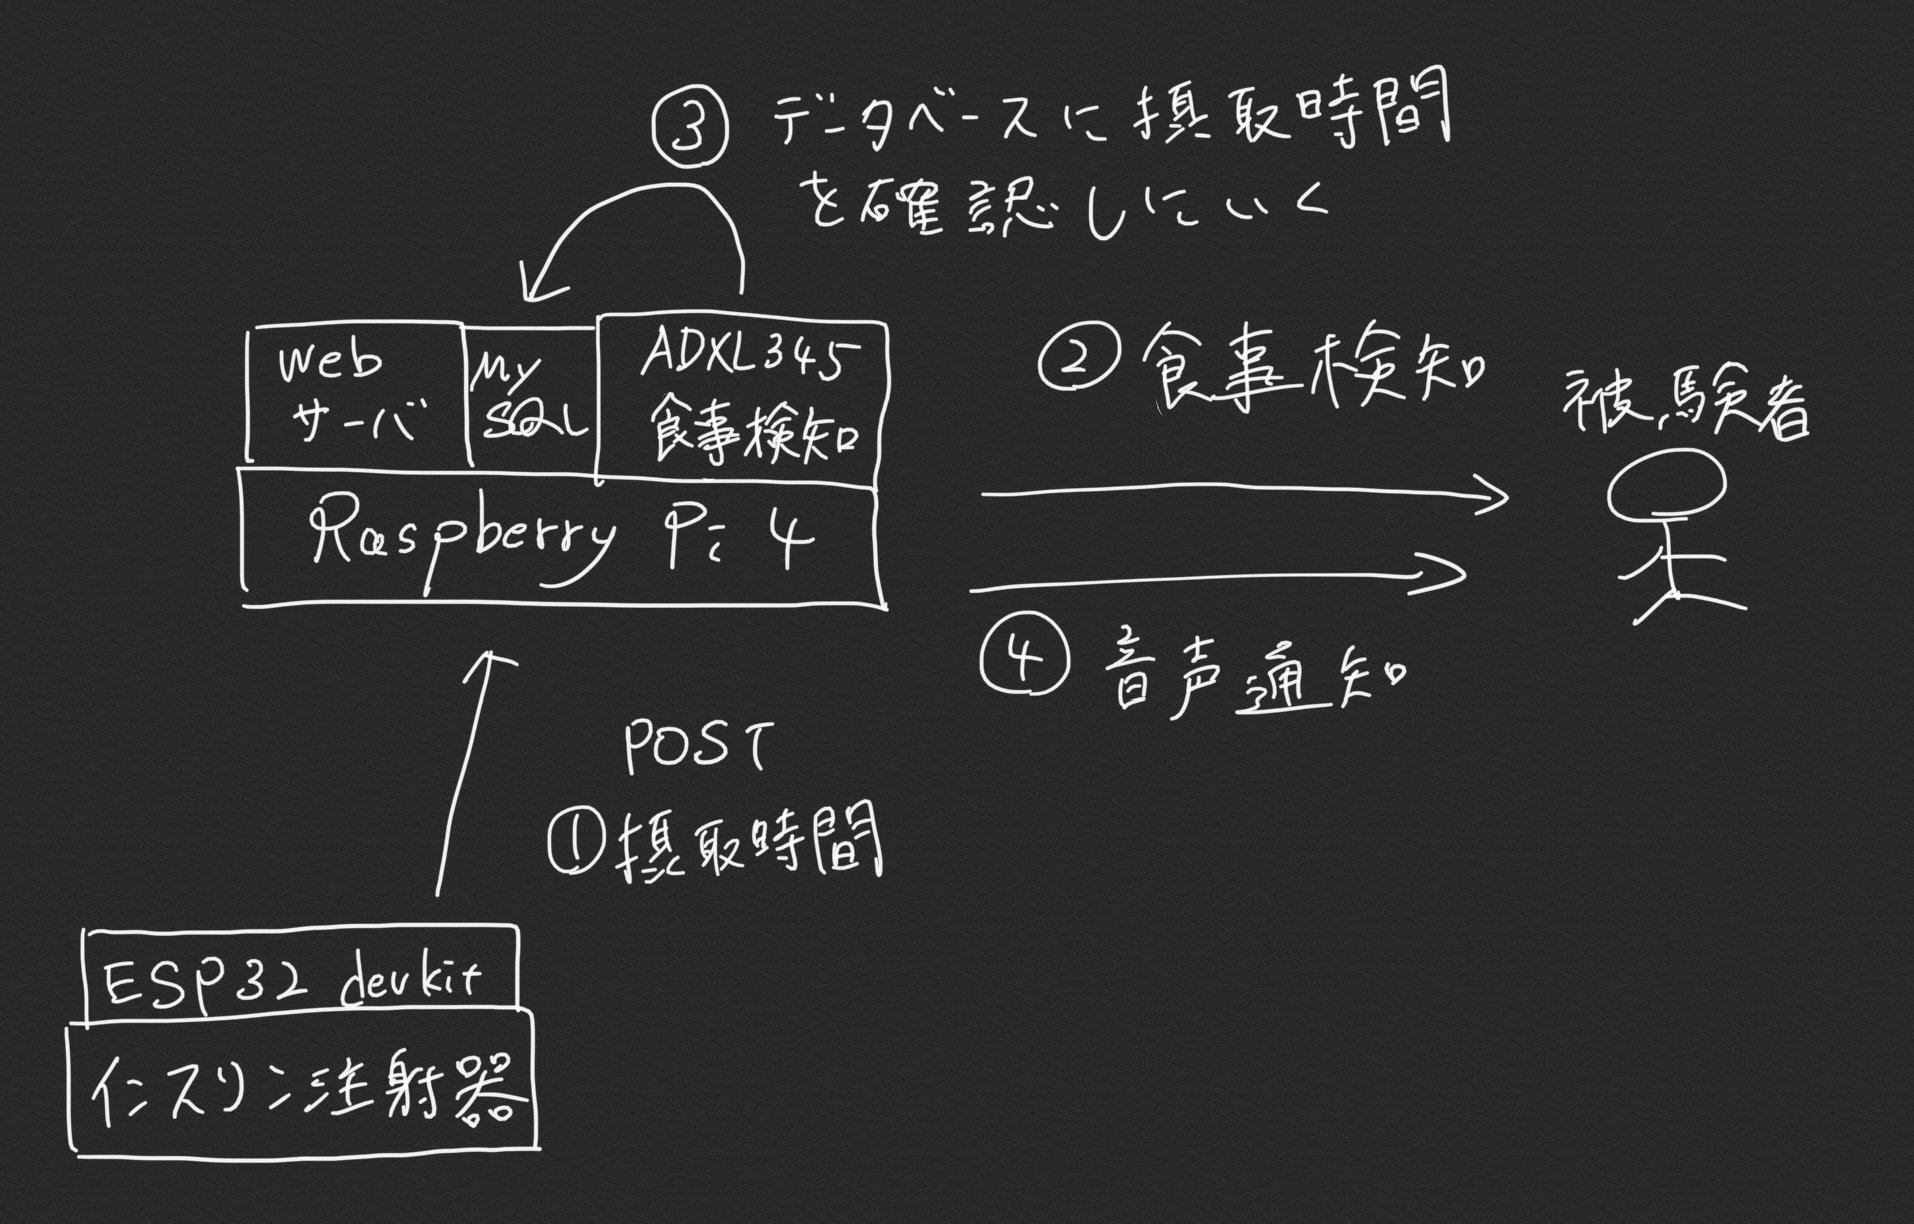
\includegraphics[bb=0 0 1000 600,width=15cm]{assets/system_flow.png}
  \end{center}
\end{figure}

% \begin{figure}[htbp]
%   \caption{}
%   \label{fig:raspi_with_speaker}
%   \begin{center}
%     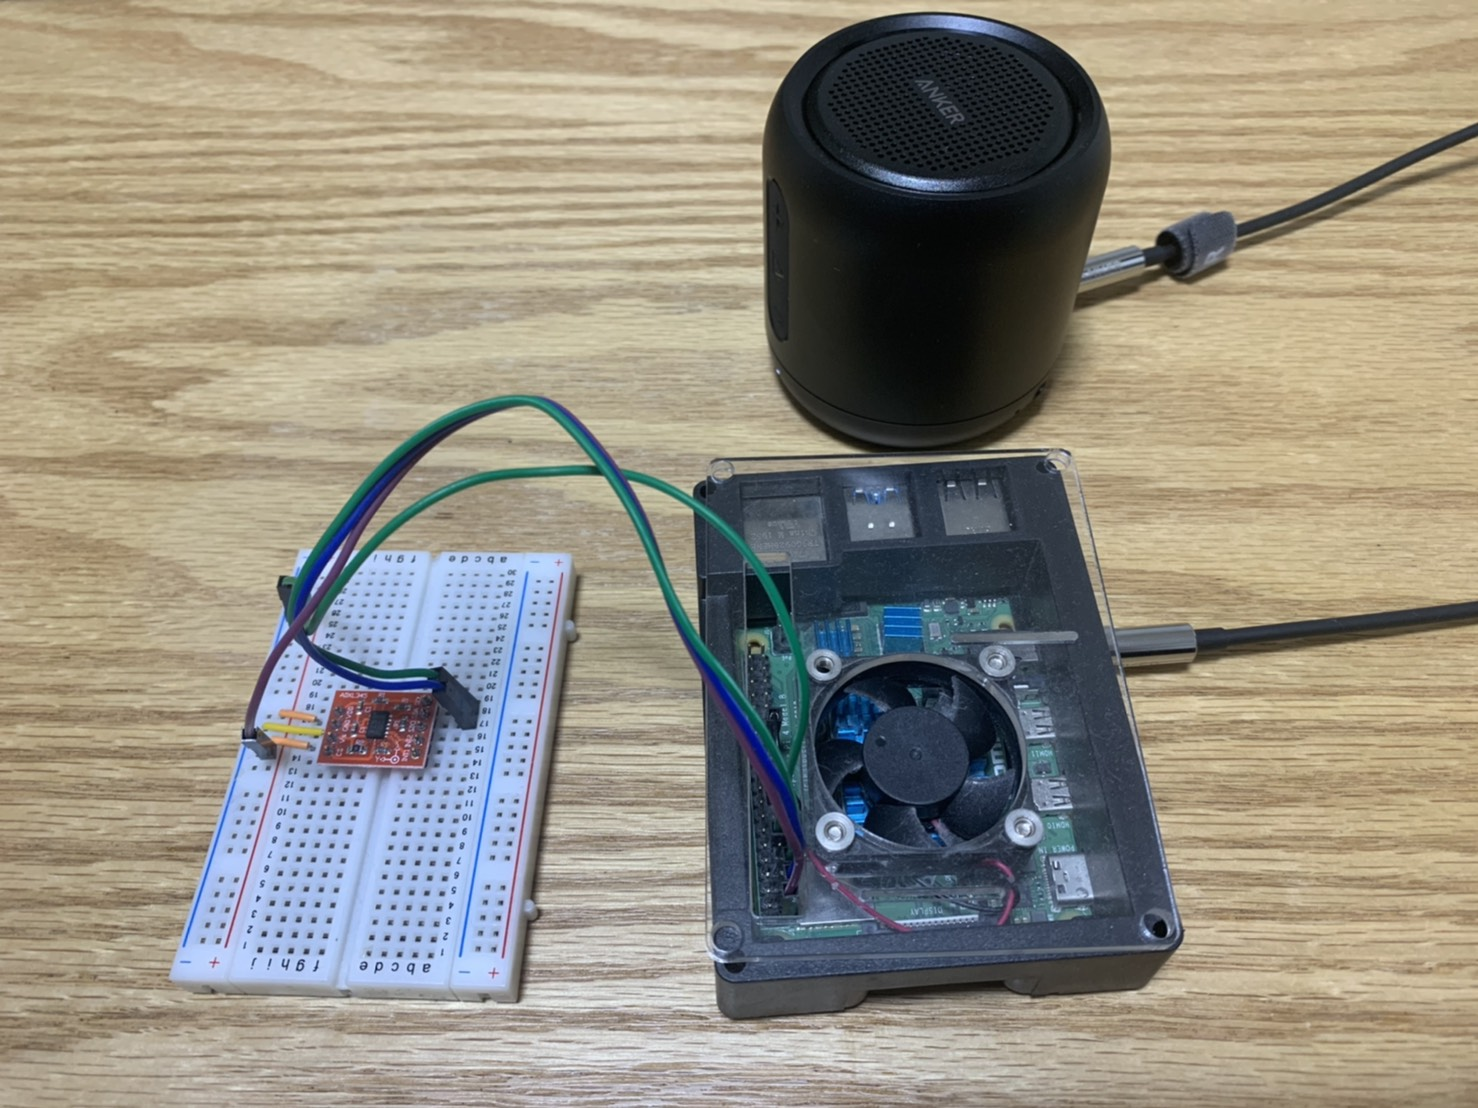
\includegraphics[bb=0 0 1000 600,width=15cm]{assets/raspi_with_speaker.png}
%   \end{center}
% \end{figure}
